
\section{Background Research}
\subsection{Types of Incongruence}
\citeA{chesney2017} talks about the differences between clickbait, fake news, sensationalism and incongruent headlines.

\subsubsection{Clickbait}
\citeA{potthast2016} define clickbait as a kind of "web content [...] designed to entice its readers into clicking an accompanying link". Clickbait uses exagerated language, outright fake information and can be accompanied by graphics designed to entice a reader. Figure \ref{fig:clickbait} shows an example of clickbait, sourced from a Natural Health website \footnote{\url{https://naturalon.com/}}.

\begin{figure}[h!]
  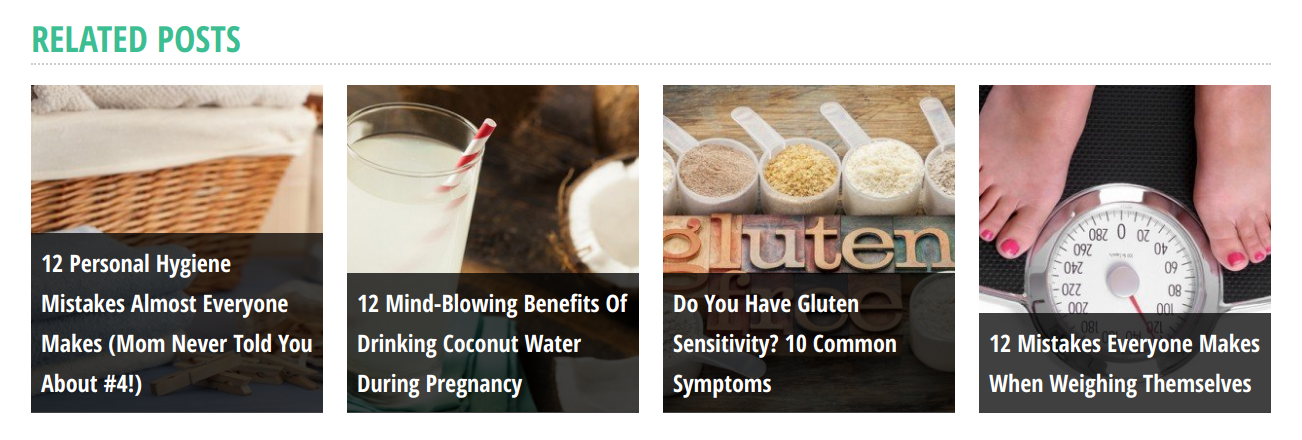
\includegraphics[width=\linewidth]{images/clickbait.png}
  \caption{Several clickbait articles in a 'chum box'}
  \label{fig:clickbait}
\end{figure}

\citeA{mahoney2015} terms a collection of clickbait stories as a 'chum boxes' - chum being dead fish used as bait for other fish. \citeauthor{mahoney2015} goes on to examine how clickbait uses pyschological methods to manipulate, an how they can have an unconcious effect on an individual.

\subsubsection{Fake News}
\citeA{allcott2017} defines fake news to be "news articles that are intentionally and verifiably false, and could mislead readers". For example, a fake news conspiracy theory claimed that a pizzeria, Comet Ping Pong, in Washington ran a child sex ring in its basement. Figure \ref{fig:fakenews} shows a news article from 2016 from Your News Wire\footnote{\url{https://archive.is/YTk3n}} (now News Punch).


\begin{figure}[h!]
  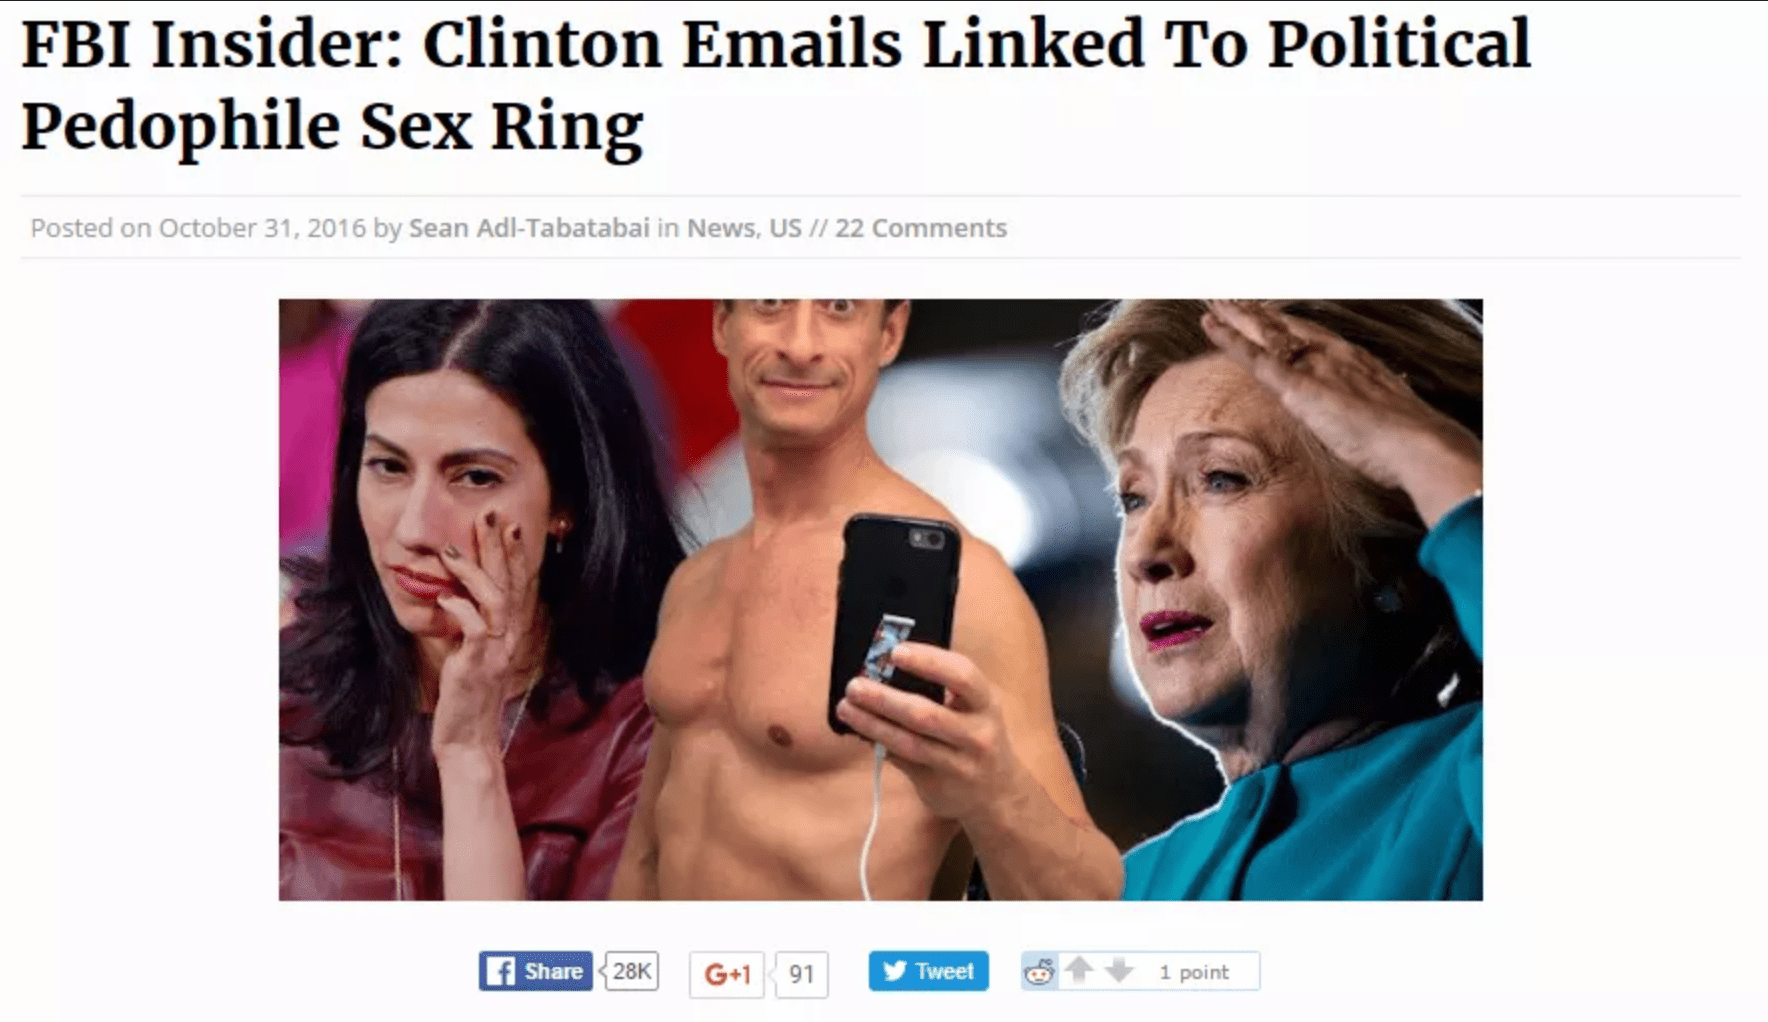
\includegraphics[width=\linewidth]{images/fakenews.png}
  \caption{A fake news story}
  \label{fig:fakenews}
\end{figure}


This lead to a man walking into Comet Ping Pong with an assult rifle and firing several shots. The restauraunt's owner and staff also recieved several death threats \cite{lopez2016}. 

\citeauthor{allcott2017} go further in their definition, and give the following sub-categories for fake news: satire, parody, fabrication, manipulation, advertising and propoganda. While the intention of satire and parody is not to decieve but to criticise, the other classifications have more subversive aims, such as misinforming people or gaining as many clicks as possible.

\subsubsection{Sensationalism}
\citeA{molek2013} defines sensationalism as "a specific discourse strategy  aimed  at  channeling  audience's  attention,  which  may  well  be  resorted  to  by  both  popular and quality outlet". They suggest that media fails to provide important and valuable news, in preference for that which is superfical and quick-paced.

Unlike clickbait headlines, information is not withheld but rather dramatised - while the aim is still to get as many clicks as possible, this is achieved through different means.

These headlines, all sourced from The Sun, are examples of sensationalised headlines:

\begin{itemize}
	\item "DOOMSDAY DISEASE FEARS Terrorists could turn ‘sniff and die’ virus that kills victims in 24 hours into a BIO-WEAPON"
	\item "SPICE UP YOUR LIFE Chilli and ginger ‘slash the risk of cancer – stopping tumours growing’"
	\item "JAB DEBATE As Melinda Messenger slams the HPV jab the parents of two teenagers blame their daughters’ ‘paralysis on vaccine’"
	\item "'I KNOW WHO KILLED JONBENET' Juror from the JonBenet Ramsey case gives sensational interview revealing he ‘knows who killed six-year-old’"
	
\end{itemize}

They use dramatic language ('slams', 'sensational', 'slash') to evoke a sense of urgency and excitement in the reader, urging them to click through to the rest of the article. 

\subsubsection{Project scope}
This project will not consider fake news - by it's nature, the entirity of a fake news article will be false, not just the headline. Therefore, in order to determine whether an article is fake, external sources would have to be consulted. Creating an algorithm for the truth, while an open problem in computer science\footnote{\url{https://www.youtube.com/watch?v=leX541Dr2rU}}, is considered out of the scope of this project.

Instead, this study will seek to evaluate to what extent a headline represents an article's body. This could identify sensationalism, over exaggerated news stories and potentially some types of clickbait.

\subsection{Impact of Incongruence}
\subsubsection{Manufacturing Outrage}
\subsubsection{}
For people who read beyond the headlines - \citeA{ecker2014} ran experiments that investigated how headlines effect the processing of the facts in news "Information that is initially accepted as valid but is later foundto be incorrect can have a persistent influence on people’s memoryand reasoning"


\subsection{Existing Approaches}
A range of studies have already considered several aspects of this project.

\citeA{manjesh2017} used Natural Language Processing (NLP) to identify 'clickbait' headlines, however they did not consider the headline's relationship to the article.

